
\chapter{Operating parameters}
\section{Forces on a car}
	\begin{wrapfigure}[8]{l}{7.5cm}
	\vspace{-5mm}
	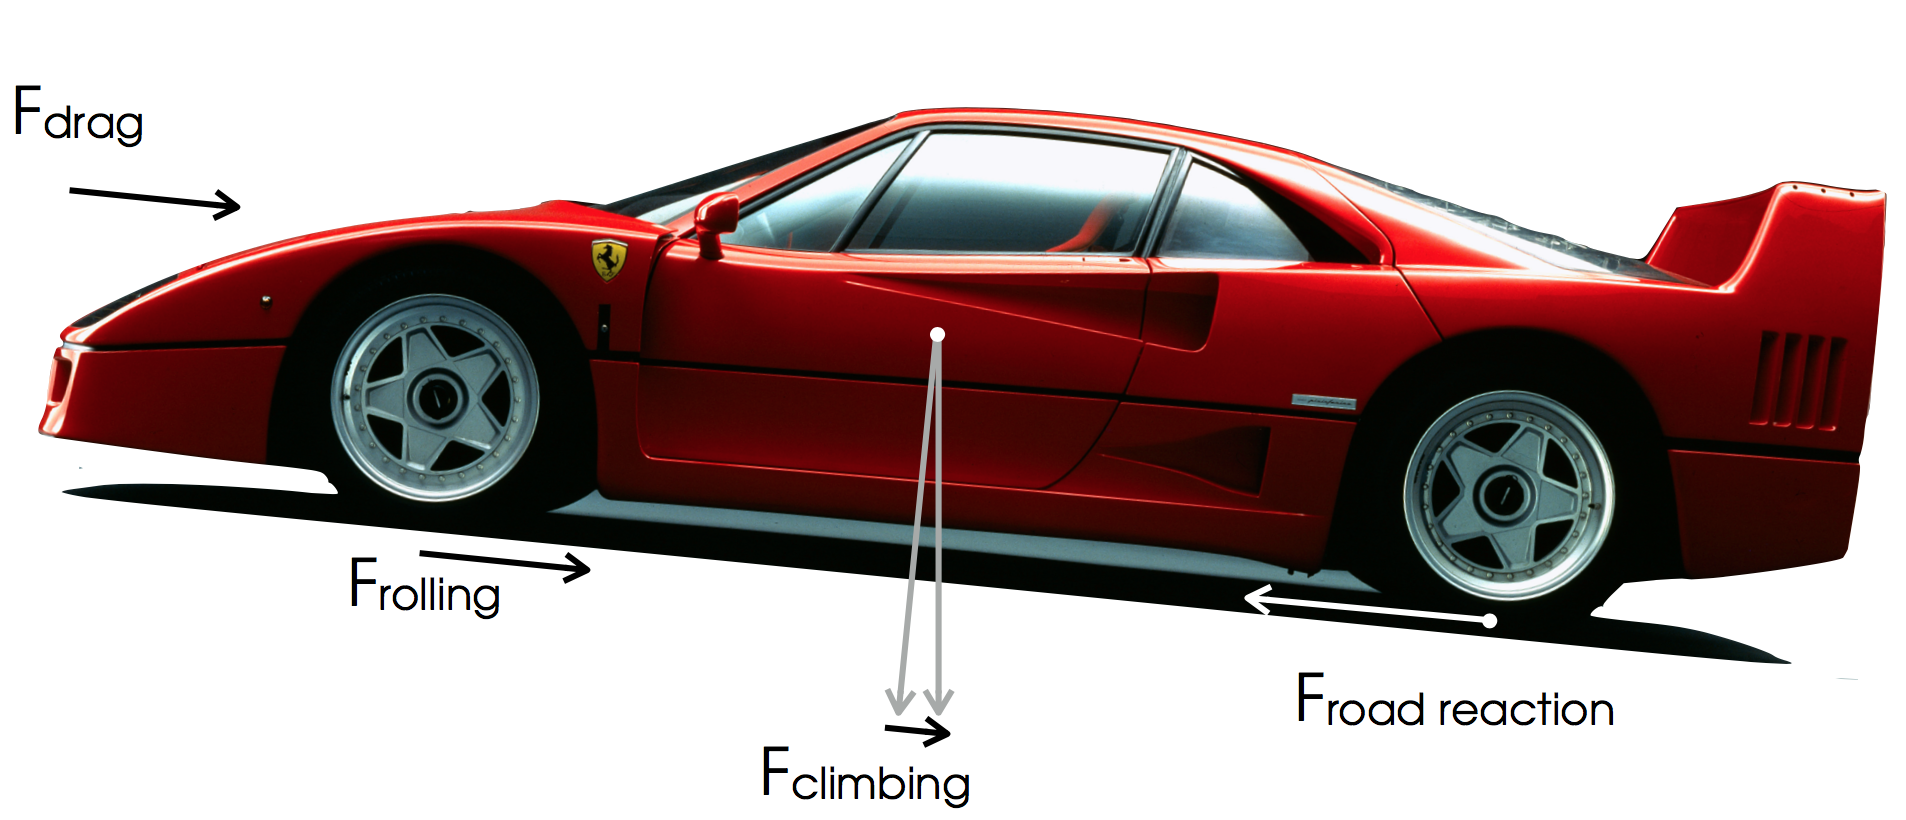
\includegraphics[scale=0.25]{ch2/1}
	\captionof{figure}{}
	\end{wrapfigure}
	The very basic, we need to apply a force to make the car move. Thus our first force is related to acceleration and energy: 
	
	\begin{equation}
	F = m.a \qquad and \qquad E= F.d
	\end{equation}
	
	This force is applied on the contact between the wheels and the road as a reaction to the torque. The three main forces opposed to the movement of the car are \textbf{rolling}, \textbf{drag} and \textbf{gravity}.
	
	